\section{Aktuálny stav} \label{sec_current}

V tejto kapitole uvedieme poznatky, ktoré sme získali po inštalovaní a spúštaní posledne dostupnej verzie robota. Rozhodli sme sa zvoliť dokončenú verziu tímu A55Kickers\footnote{\url{http://labss2.fiit.stuba.sk/TeamProject/2012/team15is-si/dokumenty/agent_robocup_fiit_v2.zip}} (\ref{A55Kickers}) %z mája 2013, pretože v čase dokončovania tejto práce\footnote{máj 2014}, prebieha vývoj v dvoch tímoch na predmete Tímový projekt - Megatroll\footnote{\url{http://labss2.fiit.stuba.sk/TeamProject/2013/team04is-si/}} a Gitmen\footnote{\url{http://labss2.fiit.stuba.sk/TeamProject/2013/team09is-si/}}. 
Postupovali sme podľa návodu na wiki\footnote{\url{http://labss2.fiit.stuba.sk/TeamProject/2013/team09is-si/wiki/index.php/Návody_a_inštalácie}}. Návod bol zrozumiteľný a pri inštalácií potrebného softvéru nenastali žiadne problémy.

Väčšinou sa pre vykonanie kopu používajú staticky definované hodnoty, ktoré sa nachádzajú v XML súbore pre pohyby. Vytváranie nového pohybu je pracné a je potrebné veľké úsilie, aby spĺňal aspoň základné vlastnosti - rýchlosť a hlavne stabilita. Aktuálne pohyby sú spracované na veľmi dobrej úrovni, optimalizované (kapitola \ref{sec_passakp}) a myslíme si, že nie je potrebné vytvárať nové.

Avšak kopy sú rovnaké a navyše kop pri inom nastavení tela hráča, ako je pozícia lopty oproti želanému smeru kopu, si vyžaduje aj prípravnú fázu, počas ktorej sa musí robot postaviť na správne miesto. Zároveň prípravná fáza zaberá dôležitý čas, počas ktorého môže súper sa dostať do vhodnejšej pozície k lopte, prípadne zablokovať strelu.

\subsection{Cieľ}

V tejto práci sme sa rozhodli implementovať parametrizovateľný a dynamický kop. Cieľom vytvorenia tohto kopu je odstrániť už spomínané nedostatky, ktoré boli spomenuté pri realizácii statického kopu. Tento kop by mal byť schopný prispôsobiť sa situácii na ihrisku a umožniť čo najpresnejšie umiestnenie lopty na požadované miesto.

Opísané svetové tímy (kapitoly \ref{austin_villa}, \ref{fc_portugal}, \ref{humboldt}, \ref{sec_bremen}) používajú okrem staticky definovaných pohybov aj pohyby dynamické. 

Aby bolo možné takýto kop používať, je potrebné implementovať taký pohyb, pri ktorom by sa za behu vypočítalo natočenie kĺbov robota. Následne by sa pohyb vykonal. Jedným zo spôsobov je použitie algoritmu portugalského tímu FC Portugal, ktorého všeobecný opis sa nachádza v kapitole \ref{fc_portugal}.

\subsubsection{Inverzná kinematika}

Inverznou kinematikou sa nazýva spôsob výpočtu umiestenia končatiny na vopred stanovenú pozíciu. Vzhľadom na to, že sa dynamickými kopmi nezaoberala žiadna práca na fakulte, je potrebné takýto modul vytvoriť. Ideálne modul, ktorý by bol použiteľný aj pre prípadné ďalšie dynamické pohyby. 

V práci Jána Hudeca\cite{hudec} je navrhnutý spôsob, ako vyriešiť tento problém. Použil by sa čiastočný prístup cez XML súbory, pričom panvové a stehenné kĺby by boli ovládané triedou \texttt{WalkControler}. Trieda by preberala údaje z \texttt{AgentModel}. \texttt{WalkControler} by si stanovil súradnice $[X,Y]$ pre pohyb a na základe nich pohne panvovými a stehennými kĺbmi. V plánovači by sa doplnil pohyb z XML súboru o pozície ostatných kĺbov nôh, príp. rúk. Obrázok \ref{pic_hudec_pohyb_activity_diag} zobrazuje diagram aktivít pre takýto prístup.

\begin{figure}[H]
	\center
	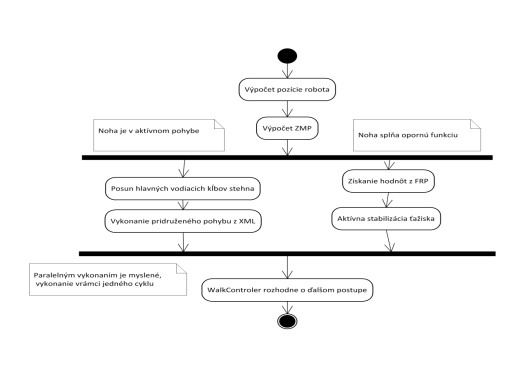
\includegraphics[scale=1]{./data/hudec_pohyb_activity_diag}
	\caption{Aktivity diagram pohybu\cite{hudec}}
	\label{pic_hudec_pohyb_activity_diag}
\end{figure}

Pre pohyb, ktorý by mal byť len dynamický je potrebné upraviť prístup Jána Hudeca a vytvoriť taký modul pre inverznú kinematiku, ktorý by dokázal určiť natočenia kĺbov pre všetky fázy pohybu bez použitia XML súborov.
 
\subsubsection{Stabilita}
%Základom každého pohybu je stabilita hráča. Každý pád môže spôsobiť aj malú časovú stratu, namiesto ktorej by sa mohol venovať hre a pokračovať vo vykonávaní svojho plánu. Ako už bolo spomenuté, pohyby sú dobré spracované a majú aj dostatočnú stabilitu. Pri vytvorení nového dynamicky meniaceho sa kopu je udržanie stability veľká výzva.
%\\
Pre statické hodnoty pohybov z XML súborov platí, že stabilita je riešená tak, že po dokončení pohybu sa musia kĺby natočiť do takej polohy, aby sa predišlo pádom. Tento prístup je pre dynamicky sa meniaci kop nevhodný.

Jedným z výsledkov diplomovej práce Jána Hudeca\cite{hudec} (kap. \ref{sec_auder_hudec}), ktorý je implementovaný vo fakultnom hráčovi JIM je použitie ZMP pre stabilizovanie chôdze.  
%toto mám priamo prebraté z Hudeca
ZMP vyjadruje, že hráč sa nachádza v zóne stability, pokiaľ kolmica na plochu zeme prechádzajúca ťažiskom robota sa nachádza v oblasti opísanej chodidlom v prípade, že hráč stojí na jednej nohe, alebo medzi oboma chodidlami, ak robot stojí na oboch nohách súčasne. ZMP počíta aj s pôsobením ostatných síl na robota - dynamika pohybu, odstredivé sily alebo gravitačná sila.

Rovnice predstavujú vzťahy pre súradnice bodu $ZMP(X_{ZMP}, Y_{ZMP}, 0)$
\begin{equation}
	X_{ZMP} = \frac{\sum_{i=1}^{n}{m_i(\ddot{Z_i} + g_z)X_i - \sum_{i=1}^{n}{m_i(\ddot{X_i} + g_x)Z_i}}}
	{\sum_{i=1}^{n}{m_i(\ddot{Z_i} + g_z)}}
\end{equation}

\begin{equation}
	Y_{ZMP} = \frac{\sum_{i=1}^{n}{m_i(\ddot{Z_i} + g_z)X_i - \sum_{i=1}^{n}{m_i(\ddot{Y_i} + g_y)Z_i}}}
	{\sum_{i=1}^{n}{m_i(\ddot{Z_i} + g_z)}}
\end{equation}

\begin{itemize}
	\item $m_i$ je hmotnosť časti tela $i$, ktorej ťažisko sa nachádza v bode $(X_i, Y_i, Z_i)$ v absolútnom karteziánskom priestore
	\item $g$ je gravitačné zrýchlenie
	\item $\ddot{X_i}$ je druhá derivácia polohy na základe času, teda zrýchlenie v danom bode
\end{itemize}

Hlavná časť implementácie sa nachádza v triede \texttt{AgentModel}, ktorá obsahuje tiež výpočty hybnosti, ťažiska, a výstupy z Force Resistance perceptora.% Ďalšou triedou je \texttt{Joint}, v ktorej sú pokročilé údaje o kĺboch.

%Pri implementácii výslednej verzie hráča som sa rozhodol použiť druhú verziu rovnice na výpočet ZMP z kapitoly 2.5.1 Zero-moment point (začiatok na strane 19) a spresniť ju pomocou hodnôt FR perceptora (ďalej len FRP – viac slovník). Na stabilizáciu využívam hodnoty oboch funkcií súčasne, na spresnenie informácii o hybnosti a pozičnej informácii hráča. JimJet je prvý z Nao robotov na našej fakulte používajúci FR perceptor na jeho stabilizáciu. Na výpočet ZMP a prispôsobenie agenta na server som vykonal úpravy a doplnenia hlavne v Java triedach: FixedObject.java – prispôsobenie hráča na nový server 0.6.5, BodyPart.java – trieda zavádzajúca podrobné informácie o modeli hráča („telesnej stavbe“) a zároveň ponúka funkcionalitu na prácu s výpočtami nad danými časťami tela (computeRelativePositionsToCamera, relativePositionToRoot, ...). AgentModel – doplnenie výpočtov hybnosti, ťažiska, ZMP súradníc, doplnenie o výstup z FRP perceptorov. Joint – doplnenie pokročilých údajov o kĺboch, úprava rozsahu efektorov, pridanie funkcionality Podrobnejšie rozobraté triedy a funkcie, ktoré som implementoval a zmeny v modeli, sú popísané v prílohe E Technická dokumentácia.

%\subsubsection{Prihrávka}
%Prihrávka spočíva v tom, že hráč, ktorý momentálne kontroluje loptu, sa rozhodne, že v danej situácii je výhodnejšia prihrávka ako priamy postup alebo strela. Následne si musí prihrávajúci hráč vybrať spoluhráča, ktorému prihrá a odhadnúť silu prihrávky a miesto, kde by mala prihrávka skončiť. Spracovanie prihrávky hráčom, na ktorého prihrávka smeruje by bolo príliš náročné a preto je lepšie vybrať pozíciu pred hráčom, kde ju môže spoluhráč následne prebrať bez nutnosti loptu zastavovať. 

%Riešenie tohto problému sa dá rozložiť na niekoľko čiastkových problémov, ktoré je následne potrebné zvládnuť na dostatočne kvalitnej úrovni, aby prihrávanie malo vôbec zmysel a prinieslo očakávanú výhodu. Prvou dôležitou časťou je už spomínané vyhodnotenie, kedy by k prihrávke malo prísť, ako aj to, kam by mala smerovať. Miesto, kam má prihrávka smerovať, musí byť pred spoluhráčom vo vzdialenosti len o čosi väčšej ako miesto, kde v momente dorazenia prihrávky bude hráč stáť. Z tohto vyplýva nutnosť zvládnuť samotnú prihrávku na takej kvalitnej úrovni, aby hráč s vysokou úspešnosťou dokázal v relatívne krátkom čase vyslať prihrávku, ktorá skončí na mieste, ktoré bude výhodné pre spoluhráča. 

%Prihrávka, ktorá by bola kratšia, dlhšia alebo nepresná, by mohla zvýhodniť súperiaci tím. Tiež je nutné pri prihrávke vyhodnocovať, či súper nedokáže prihrávku zastaviť, alebo či spoluhráč nie je tiesnení súperom a bude mať dostatok času na ďalšiu interakciu s loptou.